To estimate the feasibility of making a measurement of the 21cm-\lya\ cross-power
spectrum, it is important to define the sources of uncertainty associated with each
measurement. The noise on one particular $k$-mode in the cross-power spectrum is
dependent on noise from both the \lya\ and 21\,cm measurements, and therefore the
uncertainty from both measurements must be calculated.

I will begin by discussing the uncertainty associated with 21\,cm power
spectrum measurements due to sample variance and thermal noise. The total uncertainty
associated with an observation of the 21\,cm power spectrum can be written as follows,

\begin{equation}
\sigma_{21} \left( \textbf{k} \right) = \left[ P_{21} \left( \textbf{k} \right) + P_{21, \textrm{N}} \left( \textbf{k} \right) \right],
\end{equation}
where $P_{21}$ is the error due to sample variance and $P_{21, \textrm{N}}$ error due to thermal noise variance and is defined as,
\begin{equation}
P_{21, \textrm{N}} = X^2 Y \frac{T^2_{\textrm{sys}}}{2 t} \frac{\Omega_{\textrm{p}}^2}{\Omega_{\textrm{pp}}},
\end{equation}
where $X^2Y$ is a scalar term to convert from observed bandwidth and solid angle to $k$-mode units, $T_{\rm sys}$ is the system temperature of the array, $t$ is the observation time associated with a particular $k$-mode, determined by doing the rotation sythesis, $\Omega_p$ is the solid angle of the primary beam, and $\Omega_{pp}$ is solid angle of the square of the primary beam. More information about the parameters used in this observation can be found in Table \ref{tab:obs_table}.

In order to make the calculation of the thermal noise as realistic as possible, I use the method defined in
\cite{2013AJ....145...65P}. In this method, \textit{uv}-coverage of the observation
in taken into account using the exact layout of HERA and applying Earth-rotation
synthesis to simulate changing \textit{uv}-bins sampled by each pair of antennas.
This \textit{uv}-coverage then dictates the exact $k_{\perp}$ resolution of the instrument
while its spectral resolution sets the $k_{\parallel}$ resolution. I then perform
a spherical average over the $k_{\parallel}$ and $k_{\perp}$ bins to identify
the observation time, $t$, associated with each $k$-bin. Using this observation time
, $t$, and the equation for the thermal noise above a calculation of the 21\,cm noise power
spectrum can be made.

\begin{table}[]
\caption{Observing parameters for uncertainty calculations}
\centering
\begin{tabular}{cc}
\hline
\multicolumn{2}{c}{HERA Observing Parameters}                                                                                                                \\ \hline
\multicolumn{1}{c|}{Observing Days}                                                         & 180                                                            \\
\multicolumn{1}{c|}{Time Per Day (hrs)}                                                     & 6                                                              \\
\multicolumn{1}{c|}{Bandwidth (MHz)}                                                        & 8                                                              \\
\multicolumn{1}{c|}{Dish Size (m)}                                                          & 14                                                             \\
\multicolumn{1}{c|}{Number of Elements}                                                     & 320                                                            \\
\multicolumn{1}{c|}{$T_{\rm sys}$  (K)}                                                          & $100 + 120 \left( \nu / 150 \, \textrm{MHz} \right)^{-2.55}$ \\ \hline
\multicolumn{2}{c}{SPHEREx Observing Parameters}                                                                                                             \\ \hline
\multicolumn{1}{c|}{$x_{\rm pix} \left( '' \right)$}                                        & 6.2                                                            \\
\multicolumn{1}{c|}{$\sigma_{\rm N} \left[ \rm erg \, s^{-1} \, cm^{-2} \, sr^{-1}\right]$} & $3 \times 10^{-20}$                                            \\
\multicolumn{1}{c|}{$V_{\rm vox} \left(\textrm{Mpc}^{3} \right)$}                                         & 0.3                                                            \\
\multicolumn{1}{c|}{$\textrm{R}_{\rm res}$}                                                 & 41.5                                                           \\ \hline
\end{tabular}
\label{tab:obs_table}
\end{table}


With the 21\,cm noise power spectrum calculated above the uncertainty associated for SPHEREx can then be written similarly to the
\begin{equation}
  \sigma_{\rm Ly\alpha} = \left[ P_{\rm Ly\alpha} + P_{\textrm{Ly}\alpha, \textrm{N}} \right].
\end{equation}
Here $P_{\rm Ly\alpha}$ represents noise associated with sample variance and
 $P_{\textrm{Ly}\alpha, \textrm{N}}$ represents the thermal noise variance
on a measurement of the \lya\ power spectrum and is defined as,
\begin{equation}
P_{\textrm{Ly}\alpha, \textrm{N}} = \sigma_{\rm N}^2 V_{\text{vox}} \textrm{W}_{\rm Ly\alpha}\left(k_{\perp}, k_{\parallel}\right).
\end{equation}
In the equation above, $\sigma_{\rm N} = 3 \times 10^{-20} \ {\rm erg \ s^{-1} \ cm^{-2} \ sr^{-1}}$ (\cite{2016arXiv160607039D})
and $V_{\text{vox}}$ is volume associated a voxel measured by SPHEREx,
set by its angular and spatial resolution.
Typically the thermal noise is defined by just the first two terms, account for
the limited spectral and spatial resolution of the instrument, the thermal noise
is scaled by the window function defined in \cite{2011ApJ...741...70L},
\begin{equation}
  \textrm{W}_{\rm Ly\alpha}\left( k_{\perp}, k_{\parallel} \right) = \exp \left(\left( k_{\perp} / k_{\perp, \textrm{res}}\right)^2 + \left( k_{\parallel} / k_{\parallel, \textrm{res}}\right)^2\right).
\end{equation}
Using, the $k_{\perp}$ and $k_{\parallel}$ values set by HERA baseline lengths
and spectral resolution, I calculate the uncertainty on the \lya\ power spectrum
and spherically average to determine the sensitivity on a particular $k$-mode.
With the both uncertainty on 21\,cm and \lya\ measurements defined above, the equation
for the total variance on the cross-power spectrum can finally be defined using the equation below.
\begin{equation}
    \sigma^2_{21, \rm Ly\alpha} = \frac{1}{2} \left[ P^2_{21, \rm Ly\alpha} + \sigma_{21} \sigma_{\rm Ly\alpha} \right]
\end{equation}

Using the observational treatment and thermal noise errors defined for HERA and SPHEREx
defined above and the equation for the error on the cross-power spectrum, the cross-power spectrum
error can be calculated by again spherically averaging this 2D noise power spectrum. A plot of
the cross-terms in the cross-power spectrum can be found in Figure \ref{fig:error_budget}.
As can be seen from the figure, the cross-power spectrum, plotted in gray, turns-over
on scales that fall below the noise level. While it is encouraging that part of the cross-power
spectrum lies above the noise level, ideally a detection of this turnover would
like to be made to place constraints on the typical ionized bubble size surrounding
ionizing sources. By identifying the contributions to the cross-power spectrum error
it may be possible to develop observing strategies that make the turnover detectable.

\begin{figure}[th]
	\centering
	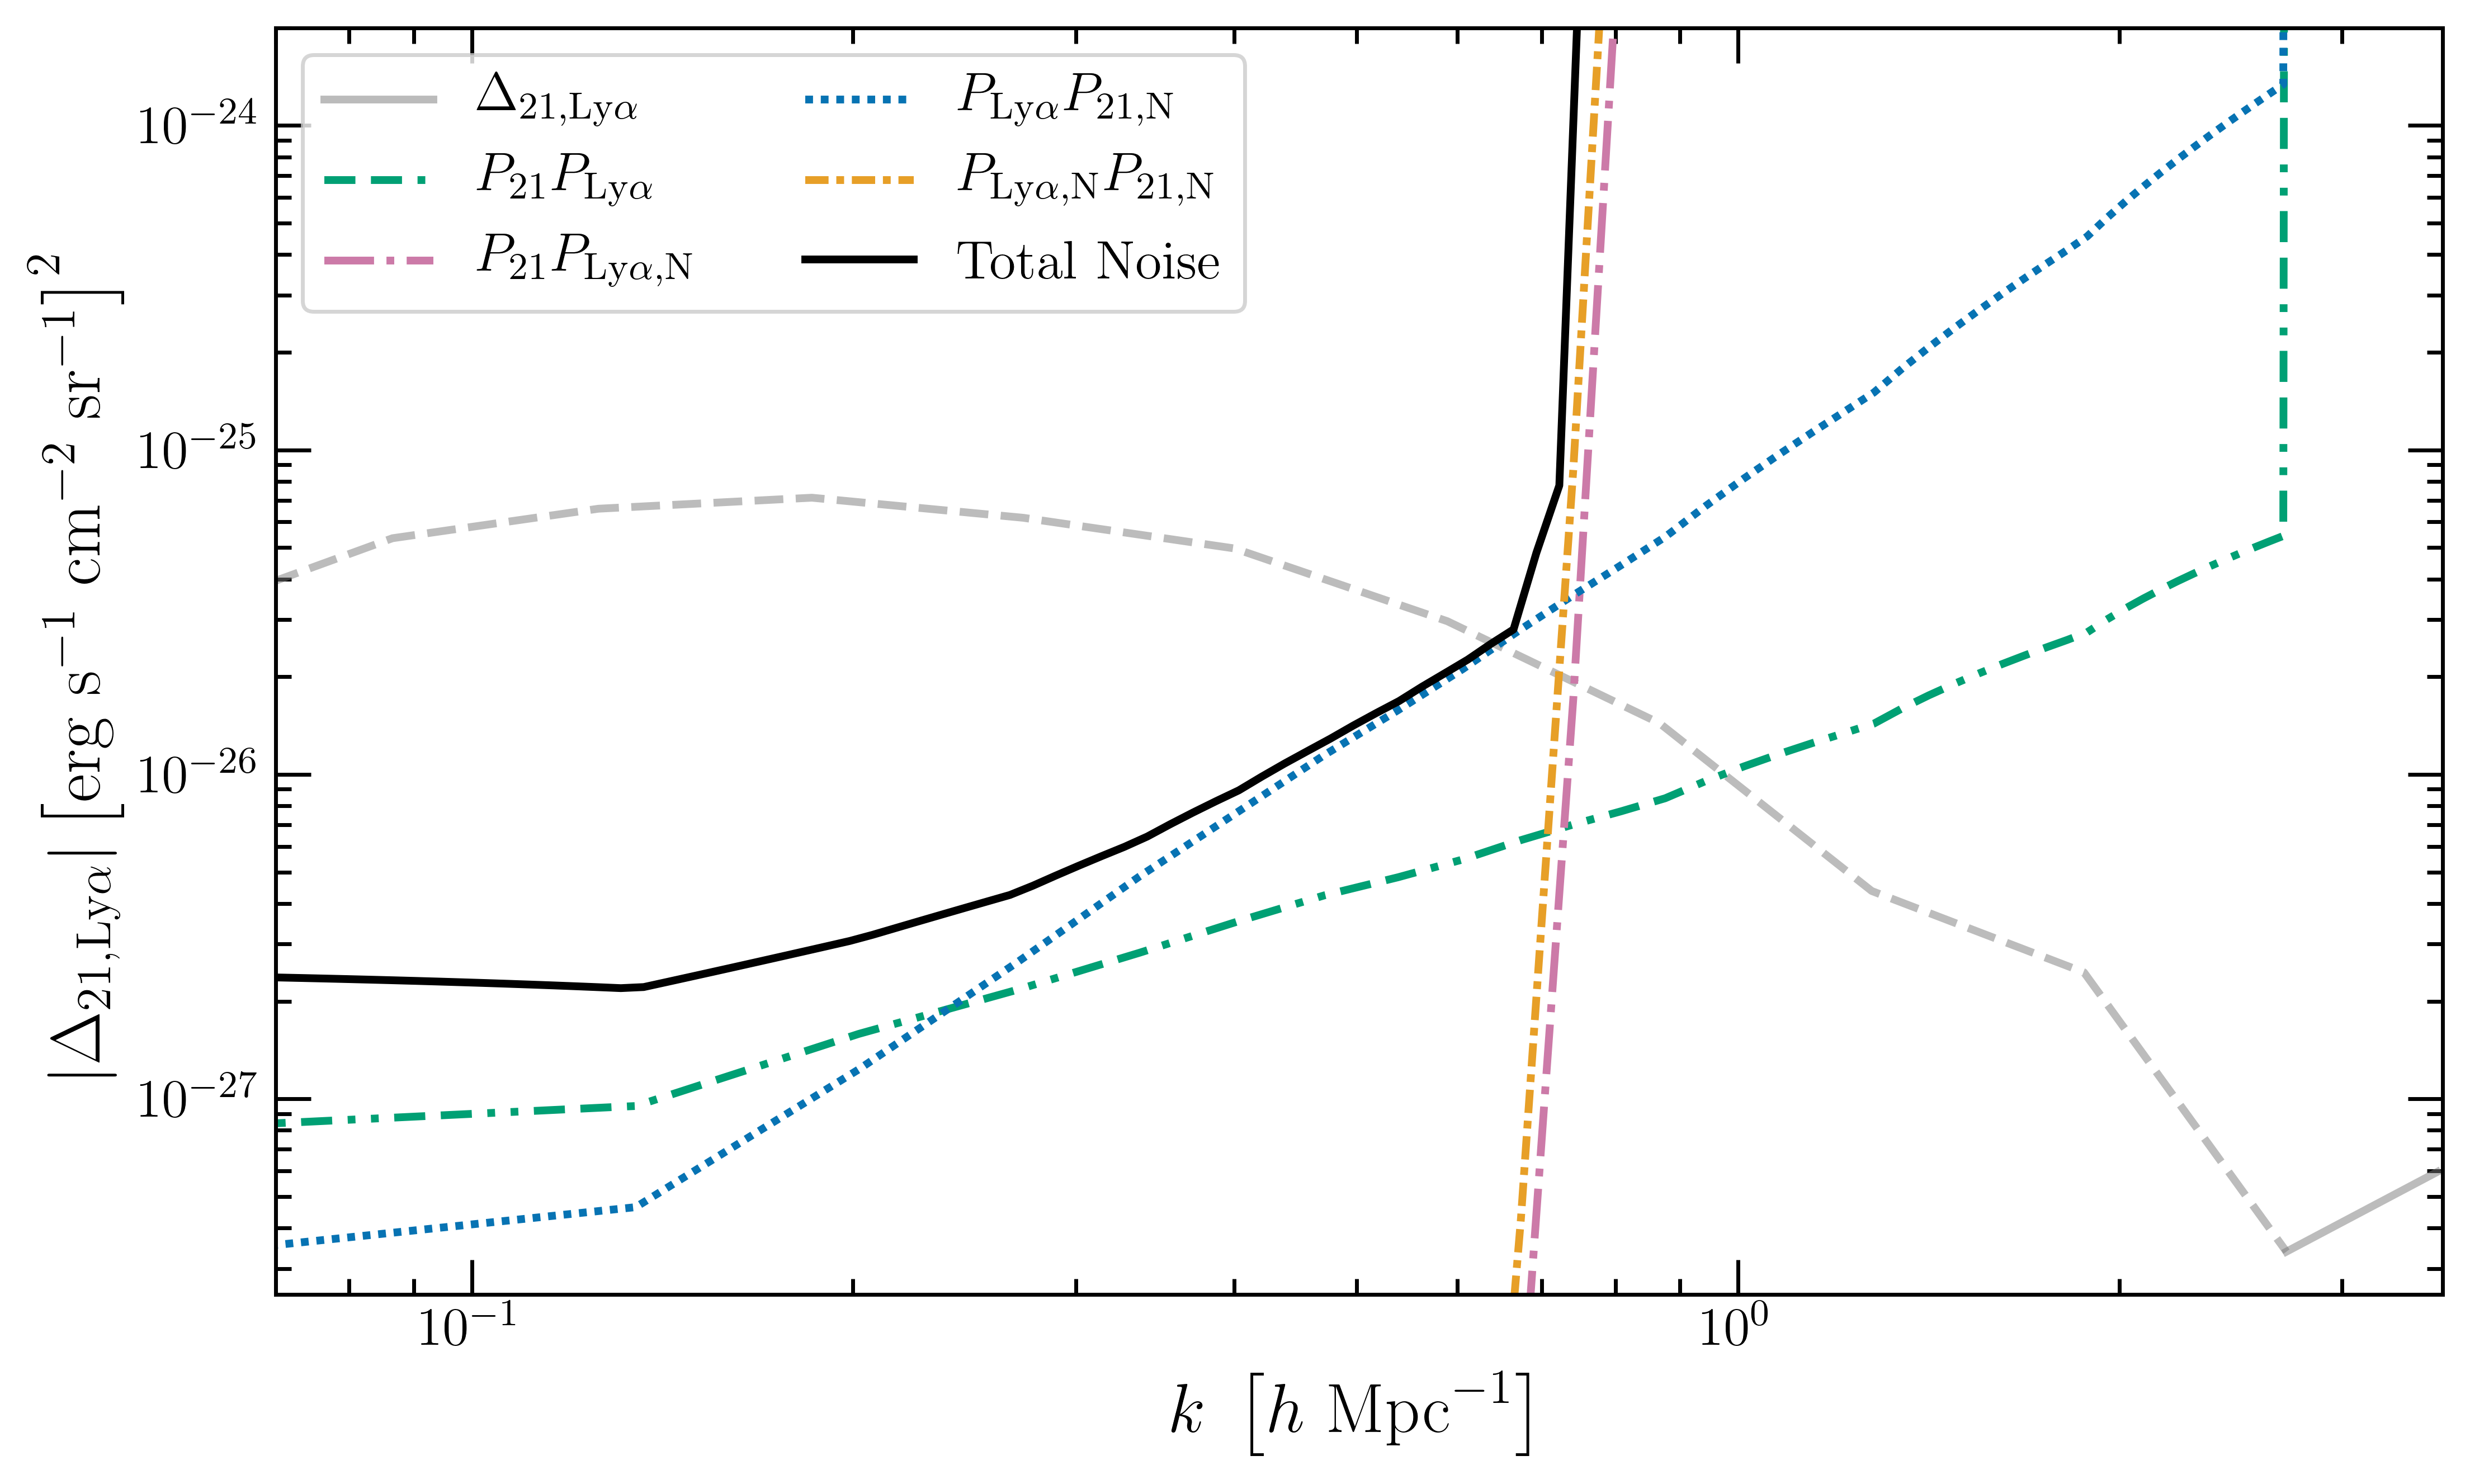
\includegraphics[width=0.95\textwidth]{error_budget.png}
	\caption[Cross-Power Spectrum Error Budget]{Error budgets of the sensitivity on the cross-power spectrum as measured by HERA and SPHEREx
  at $z = 8$ when not accounting for the foreground wedge. The terms $P_{21, \textrm{N}}$ and $P_{\textrm{Ly}\alpha, \textrm{N}}$ represent the thermal noise variance from HERA and SPHEREx respectively. Here, I neglect plotting the cross-power sample variance term, $P_{21, \textrm{Ly}\alpha }$ as its contribution is neglible, however, it is represented in the total noise of the measurement. For reference, the cross-power spectrum is plotted in gray.}
	\label{fig:error_budget}
\end{figure}

By inspecting Figure \ref{fig:error_budget}, it is obvious to see that the dominant sources of error at the scale of the turnover are the $P_{21} P_{\rm Ly\alpha, N}$ and $P_{21,\rm N} P_{\rm Ly\alpha, N}$
terms. Because both terms sharply increase at the same scales, it is safe to assume
that $P_{\rm Ly\alpha, N}$, the \lya\ thermal noise term, is responsible for the
increase due to the window function that accounts for SPHEREx's resolution limitations.
This suggests that the feasibility of this measurement is not limited by the thermal
noise contributions from either HERA or SPHEREx, but rather limited by SPHEREx's spectral
resolution. Because this limitation is a feature of the instrument itself, this tells me that
while the cross-power spectrum has the capability of being detected with a HERA-SPHEREx
cross-measurement, the turnover does not.
